%! TEX PROGRAM = pdflatex
\documentclass[a4paper]{article}

\usepackage[utf8]{inputenc}
\usepackage{microtype, listings, amsmath, amssymb, csquotes}
\usepackage{tikz}
\usetikzlibrary{arrows,shapes.geometric}

\usepackage{alphalph}
\usepackage[hidelinks]{hyperref}
\usepackage{cleveref}

\hypersetup{
    colorlinks=true
    linkcolor=red
    citecolor=green
    filecolor=magenta
    urlcolor=cyan
}



\title{Toroidal Grid Optimization via Gradient Descent}
\author{Jason Ken A}

%was node [circle,draw=black,inner sep=0pt,minimum size={width("AAA")}] {\AlphAlph{\x}\AlphAlph{\y}};}}
% was [square,draw=black]
% wassquare/.style={inner sep=0pt,minimum size={width("AA.")}
\newcommand{\toroid}[1]{
    \draw[shift={(-0.5,0.5)}] (1,-1) grid (#1+1,-#1-1);
        \foreach \x in {1,...,#1} {
            \foreach \y in {1,...,#1} {
                \node at (\x,-\y) {\AlphAlph{\y}\AlphAlph{\x}};}}
}
\newcommand{\toroidWarp}[1]{
    \begin{tikzpicture}[scale=0.8]
        \toroid{#1}
        \foreach \x in {1,...,#1} {
            \node at (\x,0) {\AlphAlph{#1}\AlphAlph{\x}};
            \node at (\x,-#1-1) {\AlphAlph{#1}\AlphAlph{\x}};
        }
        \foreach \y in {1,...,#1} {
            \node at (0,-\y) {\AlphAlph{\y}\AlphAlph{#1}};
            \node at (#1+1,-\y) {\AlphAlph{\y}\AlphAlph{1}};
        }
    \end{tikzpicture}
}

\newcommand{\toroidAxes}[1]{
        \toroid{#1}
        \foreach \x in {1,...,#1} {
            \node at (\x,0) {\AlphAlph{\x}};
        }
        \foreach \y in {1,...,#1} {
            \node at (0,-\y) {\AlphAlph{\y}};
        }
}

\newcommand{\nestedToroid}[1]{
    \begin{tikzpicture}[scale=#1]
    \draw[shift={(-0.6,0.6)}] (1,-1) grid (#1+1,-#1-1);
    \foreach \x in {1,...,#1} {
        \node at (\x,-0.25) {\AlphAlph{\x}};
    }
    \foreach \y in {1,...,#1} {
        \node at (0.25,-\y) {\AlphAlph{\y}};
    }
    \foreach \xa in {1,...,#1} {
        \foreach \ya in {1,...,#1} {
            \begin{scope}[shift={(\xa-0.5,-\ya+0.5)},scale={1/(#1+1)}]
                \toroidAxes{#1}
            \end{scope}
        }
    }
    \end{tikzpicture}
}

%
\begin{document}
\maketitle
\tableofcontents

\section{Problem Statement}%
\label{sec:problem_statement}

\subsection{Toroidal Graph}%
\label{sub:toroidal_graph}


According to \href{http://azspcs.com/Contest/Nearness}{AZSPCS}, a toroidal graph is defined as an $N\times N$ grid of unique tokens -- here presented as $IJ$, where $I$ and $J$ represent the alphabetic indices (eg. $A$ corresponds to 1) of the rows and columns respectively -- whose edges wrap around. For $N=4$, the grid is shown in \autoref{fig:toroidExample}. The tokens outside of the square grid represent tokens which ``wrap around'' the grid (hence the toroidal grid).
\begin{figure}[htpb]
    \centering
    \toroidWarp{4}
    \caption{A $4\times 4$ toroidal grid}%
    \label{fig:toroidExample}
\end{figure}

\subsection{Evaluation Function}%
\label{sub:evaluation_function}

The goal of the challenge (and hence this essay) is to create a new grid -- with tokens allowed to be arranged in any order -- which minimizes a loss function (how much it fails) defined as follows:
\begin{enumerate}
    \item For each pair of tokens, calculate the squared distance between them in the new grid,
\item multiply it with its squared distance within the original grid
\item The sum of these multiplications is the value of the loss
\end{enumerate}
As is with all loss functions, the goal is to minimize the loss function.

\subsubsection{Distance Metric}%
\label{ssub:distance_metric}
If 2 two-dimensional coordinates are defined as $s_1=(x_1,y_1)$ and $s_2=(x_2,y_2)$, the Euclidean distance $d$ is defined as

\begin{equation}
    \label{eq:euclid}
    d(s_1,s_2)=\sqrt{(x_2-x_1)^2+(y_2-y_1)^2}=\sqrt{(\Delta x)^2+(\Delta y)^2}
\end{equation}

and the squared Euclidean distance $d^2$ evaluates to
\begin{equation}
    d^2(s_1,s_2)=(\Delta x)^2+(\Delta y)^2
    \label{eq:squaredEuclid}
\end{equation}
simplifying much of the computation.

But with a toroidal surface, both $\Delta x$ and $\Delta y$ have 2 possible values. A one-dimensional case with toroidal surface of length $N$ is shown in \autoref{fig:2distanceexample}. These two distances can be written as

\begin{figure}[htpb]
    \centering
    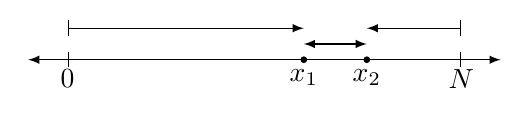
\begin{tikzpicture}
        \draw[latex-latex] (-3,0) -- (3,0);
        \draw[|-|] (-2.5,0) node[below] {$0$} -- (2.5,0) node[below] {$N$};
        %\draw[|-|] (-2.5,-0.5) -- node[below] {$N$} (2.5,-0.5);
        \filldraw (0.5,0) circle (1pt) node[below] {$x_1$};
        \filldraw (1.3,0) circle (1pt) node[below] {$x_2$};
        \draw[latex-latex] (0.5,0.2) -- (1.3,0.2);
        \draw[latex-|] (1.3,0.4) -- (2.5,0.4);
        \draw[|-latex] (-2.5,0.4) -- (0.5,0.4);
    \end{tikzpicture}
    \caption{One-dimensional diagram of toroidal distance}%
    \label{fig:2distanceexample}
\end{figure}


\begin{align*}
    %\label{eq:naiveToroidDistance}
    \Delta_1(x)&=x_2-x_1 \\
    \Delta_2(x)&=(x_1-0)+(N-x_2)=x_1+N-x_2
\end{align*}

To obtain a general equation which works with both $x_1>x_2$ and $x_1<x_2$, we can write
\begin{align*}
    \Delta_1(x)&=\lvert x_2-x_1 \rvert \\
    \Delta_2(x)&=\min{(x_1,x_2)}+N-\max{(x_1,x_2)}
    %\label{eq:absoluteToroidDistance}
\end{align*}
where $ \lvert a\rvert$ is the absolute value of $a$, $\min{(a,b)}$ and $\max{(a,b)}$ are defined as the minimum and maximum of $a$ and $b$ respectively. $\min$ and $\max$ are used to determine the  ``left-most'' and the ``right-most'' numbers.

Since, the distance can only have 1 value, it is defined as
\begin{align*}
    \Delta x=\min{(\Delta_1(x),\Delta_2(x))}
\end{align*}

Generalizing it to 2 dimensions, we get
\begin{align*}
    d(s_1,s_2)&=\sqrt{(\Delta x)^2+(\Delta y)^2} \\
    d^2(s_1,s_2)&=(\Delta x)^2+(\Delta y)^2 \\
\end{align*}
where $d^2$ is the distance metric to be used in our calculations.

With $U$, $O$, $D$, $T$, defined an upper triangular matrix filled with ones, and the flatenned matrix of the original grid, modified grid, and set of all tokens, respectively. The loss function can be written as
\begin{align*}
    \label{eq:evaluationFunction}
    %L(O)=\sum_i^{n(T)}{\sum_{j,j\geq i}^{n(T)}{d^2(O_i,O_j)\cdot d^2(D_i,D_j)}}
    L(O)=\sum_i^{n(T)}{\sum_{j}^{n(T)}{d^2(O_i,O_j)\cdot d^2(D_i,D_j)\cdot U_{ij}}}
\end{align*}
% still explain how to unravel a matrix

where the double summation enables calculating every possible combination of pairs, and $U$ removes duplicate entries (eg. [$AA$, $AB$] and [$AB$, $AA$]).

\section{Superposition}%
\label{sec:superposition}
Since the entries into the toroidal grid are discrete (eg. $AA$ can only be in one position), it is not possible to optimize the loss function. Therefore, relaxing the constraints to enable superposition -- here defined as having a token being in multiple positions at once each with its own ``probabilities'' -- is essential.

A simple method of allowing superposition, is by allowing any position to have any token value

%\toroidAxes{3}
\nestedToroid{2}
\end{document}
